%!TEX root = ../Touch Based Idris.tex
\section{Implementation}
\label{sec:Implementation}

Having the architecture marked down, we could focus on another iteration of
usability testing. It was the goal to create a prototype running on the iPad,
ready for usability testing with a bigger group of participants than in the
mock-up phase.

\begin{figure}
	\centering
		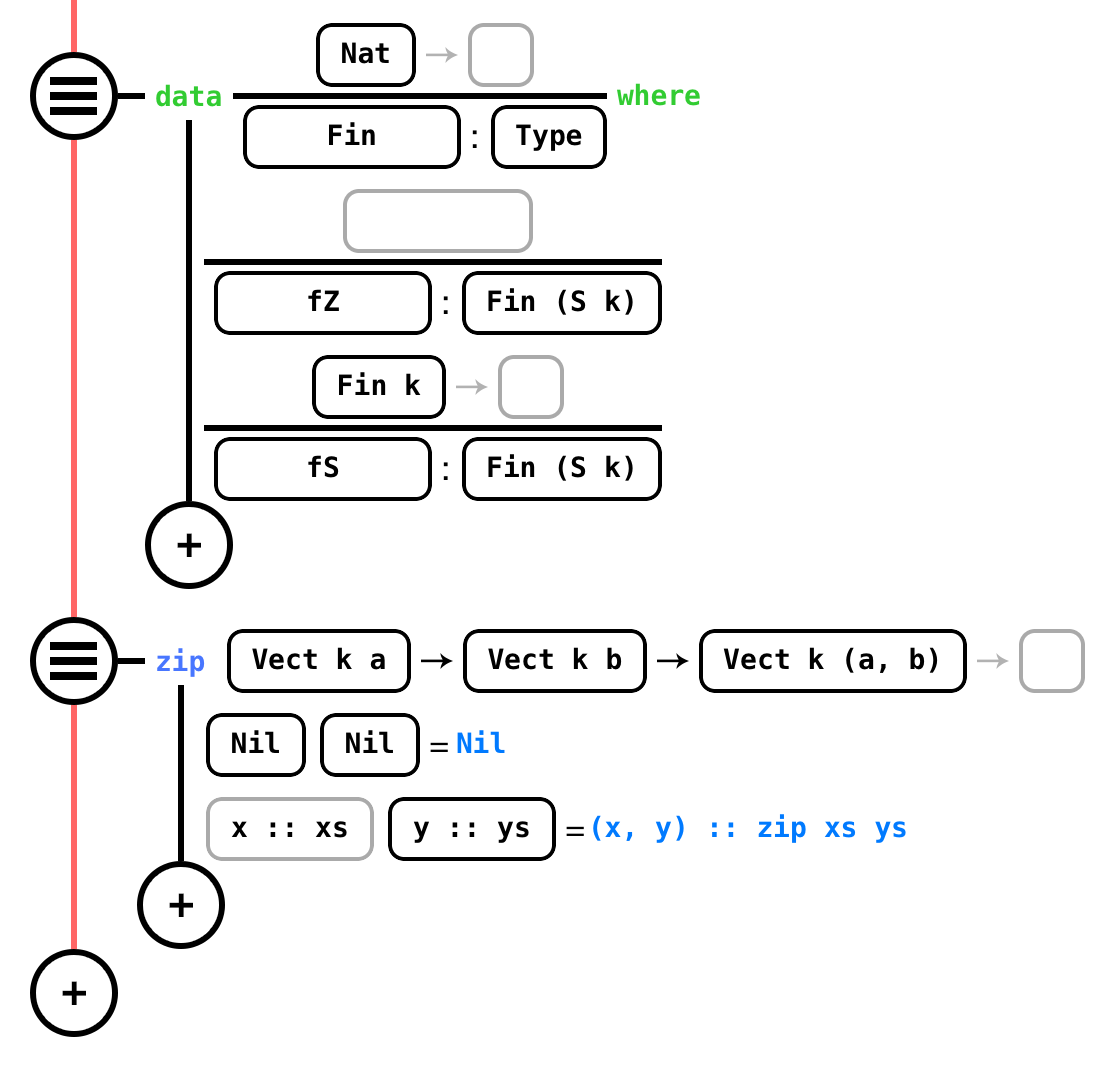
\includegraphics[width=110mm]{diagrams/ipad_interface.PNG}
	\caption{The initial iPad interface.}
\label{fig:initialiPadInterface}
\end{figure}

\begin{figure}
	\centering
		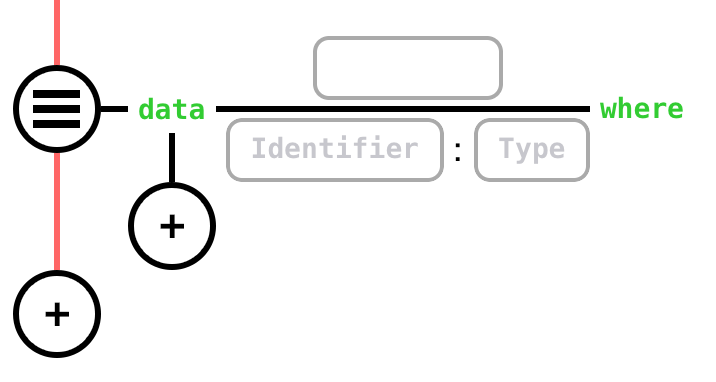
\includegraphics[width=70mm]{diagrams/data_declaration.png}
	\caption{A data declaration before the user has filled out anything.}
\label{fig:data_declaration}
\end{figure}

To produce this prototype we had to follow the usability recommendations of
Section~\ref{sec:first_recommendations}	while still keeping the goals and requirements of
Section~\ref{sec:GoalsAndRequirements} in mind. Figure~\ref{fig:initialiPadInterface}
shows an example data type as well as the zip function defined in the visual,
high-level syntax. It is evident that this is still a prototype, but the reader
should be able to get an idea of how it works.

One of the things that were not implemented in the initial prototype was the
TouchDevelop-like focus shifting, where different top-level elements would be
in focus at different times. In this prototype all elements are in focus all
the time.

The data declarations (see Figure~\ref{fig:data_declaration}) were kept the same as in the mock-up except for the
placeholder text and colon indicating the separation between the identifier and
type.

This prototype consists of a lot of custom elements, and the way that they work
together has been challenging to implement. Figure~\ref{fig:clientViewArchitecture} shows a simplified class diagram of the
client. It shows the UI classes of the project to give an idea of
the resemblance to the abstract syntax. As with the abstract syntax there are
two ``levels'' of views --- top level and input level. The MainView holds a
number of top level declarations, that each hold a number of input views. The
InferenceRuleView is used by the DataDeclarationView only.

A GroupInputView contains one or more AbstractInputViews. This way of building
the interface makes it easy to wire input views to the underlying model object
hierarchy, as it is the same type of nesting we have with terms. \todo{Explain
what the group input view is and how it can be customized}

\begin{figure}
	\centering
		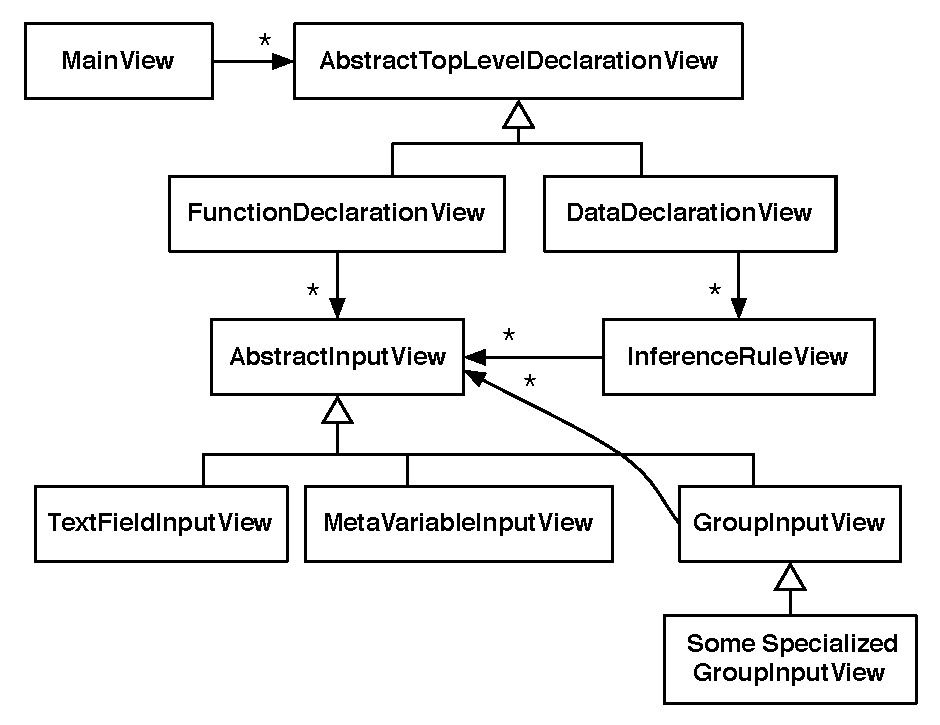
\includegraphics[width=110mm]{diagrams/client_side_class_diagram.pdf}
	\caption{A subset of the client-side diagram showing how the view hierarchy
	almost mirrors the Abstract Syntax tree.}
\label{fig:clientViewArchitecture}
\end{figure}

\subsection{Second Usability Iteration}
\label{sec:SecondUsabilityTest}
The greatest change in the second usability test was the fact that it was
performed on an actual iPad, using a prototype interface. The full report is
included in Appendix \todo{insert ref}. As in the first test, S2.4 refers to
the fourth point in the test summary for subject 2.

\subsubsection{Participants}
For our second usability test, we used two subjects from the first test,
subject \#1 and \#2. Their input was interesting, as they already had some
experience with the ideas in our representation from the mock-up test.
Hopefully this would let them focus more on the interactions with interface,
and less on learning a new way of presenting data. Subjects \#3 and \#4 had
never seen the interface before, and as such represented totally new users.
Their feedback was also very useful, as this iteration tried to make the first
time experience less frustrating.

\begin{table}[h]
\centering
\begin{tabular}{| l | l | p{5cm} | p{5cm} |}
\hline
Subject & Age & Occupation & Experience \\ \hline
\#1 & 24 & Masters student at IT-University studying programming languages & 7 months experience with Idris, several years of experience with functional languages in general \\ \hline
\#2 & 27 & Masters student at IT-University studying programming languages & 7 months experience with Idris, several years of experience with functional languages in general \\ \hline
\#3 & 27 & Masters student at IT-University studying programming languages & Very little experience with Idris. 1 year experience with Coq. Several years of experience with functional languages in general \\ \hline
\#4 & 23 & Masters student at IT-University studying programming languages & 6 months experience with Idris. Several years of experience with functional languages in general \\ \hline
\end{tabular}
\caption{Test subjects}
\label{table:second_test_subjects}
\end{table}

\subsubsection{Session Details}
Like the first test, this test was conducted in a meeting room at the IT
University, with three people present: The test subject, the test facilitator,
and a note taker. The tests were recorded. This time the test consisted of four
tasks, with the first task designed to get the subjects acquainted with the
data declarations. The next two tasks were identical to the first test, the
definition of the \texttt{Vect} data type and the \texttt{zip} function for
\texttt{Vect}. The final task concerned the manipulation of order of
declarations in the program they defined. As the app was still at prototype
stage, several bugs occurred during the subjects' use of the app. In these
cases the nature of the bug was quickly explained, and the facilitator
explained how to work around the issue.

\subsubsection{Tasks}
The four tasks they were asked to complete are listed in 
Figure~\ref{figure:second_tasks}.
As in the first test, the test subjects had access to the definitions for
\texttt{Vect} and \texttt{zip} textual Idris. See Section~\ref{subsec:Idris}
for more on \texttt{Vect} and \texttt{zip}.

\begin{figure}
\centering
\begin{itemize}
	\item \textbf{Task 1}: The user is shown the \texttt{Nat} and \texttt{Fin} data declaration in the program.
	\begin{itemize}
		\item \textbf{T1.1}: Describe the \texttt{Nat} type.
		\item \textbf{T2.2}: Describe the \texttt{Fin} type.
	\end{itemize}
	\item \textbf{Task 2}: Define a data declaration for the vector type.
	\begin{itemize}
		\item \textbf{T2.1}: Specify an identifier for the type (\texttt{Vect}), along with its type (\texttt{Nat -> Type -> Type})
		\item \textbf{T2.2}: Specify the Nil constructor (\texttt{Nil: Vect z a})
		\item \textbf{T2.3}: Specify the Cons constructor (\texttt{(::): a -> Vect k a -> Vect (S k) a})
	\end{itemize}
	\item \textbf{Task 3}: Define the zip function for vector type.
	\begin{itemize}
		\item \textbf{T3.1}: Specify the identifier for the function (\texttt{zip}), along with its type (\texttt{Vect k a -> Vect k b -> Vect k (a, b)})
		\item \textbf{T3.2}: Specify the first case (\texttt{zip Nil Nil = Nil})
		\item \textbf{T3.3}: Specify the second case (\texttt{zip x::xs y::s = (x, y) :: zip xs ys})
	\end{itemize}
	\item \textbf{Task 4}
	\begin{itemize}
		\item \textbf{T4.1}: Move the \texttt{Vect} declaration up below \texttt{Nat}.
	\end{itemize}
\end{itemize}
\caption{Tasks for the second usability test. The text in parentheses are what we considered the correct answer, and was not given to the test subjects.}
\label{figure:second_tasks}
\end{figure}

\subsubsection{Issues}
\label{sec:second_issues}
Many new issues were discovered in this usability test. This is not
surprising. In the first test, the facilitator took over the iPad's role, by
manipulating the mockups. This masked many flow and ease of use issues, which
have now been identified. During the test, several bugs were encountered. These
are not listed below, as they are not inherent to the design, but rather
results of the prototypical nature of the app.
\\ \\
\textbf{I1: Too many input fields}.
Most of the users reported that all the grey, unfilled input fields were
confusing. (S1.20, S2.2, S3.29b)
\todo{Insert screenshot}
\\ \\
\textbf{I2: Writing data declaration}
Everyone was able to decipher the data declarations almost immediately, but
all but one had trouble writing the \texttt{Vect} data declaration. Especially
the distinction between the premise area and the conclusion area seemed
problematic. (S1.1--1, S3.11--18, S4.3--7)
\\ \\
\textbf{I3: Arrows in data confusing}
The use of arrows in the premise area is confusing, as it implies a function. 
(S4.4)
\\ \\
\textbf{I4: Suggestions for parameterized types}
This issue persists from the original design. The subjects found it irritating
that after choosing a suggestion, they would have to manually change the
parameters using the standard iOS text editing facilities. Multiple subjects
mentioned that it broke their flow. (S1.10, S2.7, S3.15)
\\ \\
\textbf{I5: Lack of auto-closing parentheses and quotation marks}
We observed that users spent too much time navigating the virtual keyboards to
close pairs of symbols, when this can be done automatically.
\\ \\
\textbf{I6: Common symbols inaccessible}
In a similar vein, we noticed that some symbols commonly used when programming,
e.g. ``<'', took too long to find in the virtual keyboard.
\\ \\
\textbf{I7: Poor flow between input fields}
To move from one input field to the next, the subjects must manually tap each
input field. This broke the subjects flow. (S1.21, S3.30c)
\\ \\
\textbf{I8: Program can look cluttered}
After finishing all the tasks, the subject's program started to look cluttered.
\todo{Insert screenshot} (S3.29a)
\\ \\
\textbf{I9: Few definitions visible}
Related to Issue I8, definitions are quite large, so only a few are visible at
any time. This can make it hard for the subject to get an overview of their
work.
\\ \\
\textbf{I10: Unclear how to specify implicits and identifiers for arguments}
Some parts of the syntax have not been determined. Some of the subjects
wondered how one would make an argument implicit. (S1.9, S4.13)

\subsubsection{Recommendations}
\label{sec:second_recommendations}
As this represents the final iteration during this project, these
recommendations serve more as a reflection over how these issues might be
addressed.\todo{Ref to section with more reflection}

\begin{itemize}
    \item \textbf{Re1} (I1): Differentiate input fields to a greater degree. Perhaps outline required input fields in red, to differentiate them from other input fields.
    \item \textbf{Re2} (I1): Do not show input fields for declarations that don’t have focus.
    \item \textbf{Re3} (I1): When centering text that includes an extra input field, center the text without the input field. \todo{Insert screenshot}
    \item \textbf{Re4} (I3): Use semicolons instead of arrows.
    \item \textbf{Re5} (I4): When showing types that take parameters, indicate these parameters in the popup. Then, after choosing one, create two new sub input fields, with their own autosuggestions. Make sure theres a good flow between these fields.
    \item \textbf{Re6} (I5): Automatically close pairs of symbols.
    \item \textbf{Re7} (I6): Include a (customizable) shortcut bar for symbols.
    \item \textbf{Re8} (I7): After filling a field, automatically move input to next field. Perhaps include a button to move back and forth between fields.
    \item \textbf{Re9} (I8): Include more spacing between fields.
    \item \textbf{Re10} (I9): Include a cheat sheet on the right hand side, showing constructors and types for functions.
    \item \textbf{Re11}: In general, it might be good to separate text editing from general manipulation of the program. Text editing could occur in popups or a dedicated text input field, freeing gestures for other uses when manipulating the structure of the program.
\end{itemize}

\todo{sub section conclusion}

\subsection{New Design}



\subsection{Next Usability Iteration}
With this new design we feel that the user interface has reached a maturity
level where it is important to focus on the server-side for a while. In the
next usability test, the solution's edit-compile-test cycle should be tested to
a larger extent, and that requires a working back-end. The following usability
test cases assume that we have a working prototype with the new design
implemented as well as a working server that can serve compilation results.

The participants of the usability test should again be a mix of programmers
that are new to the platform and some that are not. Other than that, they
should be screened in the same way as in our second usability test (Section
\ref{sec:SecondUsabilityTest}).

What we specifically wish to test in this next usability test is:

\begin{enumerate}
	\item The flow when declaring new data types and functions. This includes the auto-completion feature and the context popover
	\item The understandability of the way we now declare data types
	\item The focus system, where only one top-level declaration is in focus at a
	time. Can users maneuver in and out of declarations in a fairly easy way?
	\item Editing right-hand sides that have already been added.
	\item Deleting terms by flicking them and rearranging them by dragging.
	\item Deleting top-level declarations, clauses, and constructors
\end{enumerate}

It does not make sense to draw up an exact usability test plan like the ones we have made in previous usability
at this point. We would need to have a working version of the solution before a precise test plan can be made. Also, the few points listed above could easily amount to more than 10 tasks, which is more than can be completed in an hour with a participant. For this reason we would have to prioritize the focus of the test, and that can only be done when we have the new solution in our hands and decide what features we are most confident about. 

















